\documentclass{beamer}
\usepackage[spanish]{babel}
\selectlanguage{spanish}
\usepackage[utf8]{inputenc}
\usepackage{hyperref}
\usepackage{graphicx}
\usepackage{float}


\usetheme{Frankfurt}
\usecolortheme{whale}

\title{Conceptos de Git}
\author{Emmanuel Arias \href{mailto:emmanuelarias30@gmail.com}{emmanuelarias30@gmail.com}}
\date{}
\begin{document}
\begin{frame}[plain]
    \maketitle
\end{frame}

\begin{frame}
   \Huge Git Internals
\end{frame}

\begin{frame}{Git Internals}
	\begin{itemize}
		\item En git los archivos se almacenan en archivos \textbf{blobs} (binary large objects)
		\item La ventaja de usar estos Blob y un archivo normal es que estos últimos guardan metadata. En cambio los Blobs es solo contenido.
		\item Cada blob es identificado por un código has SHA-1. 
		\item En Git cada directorio o carpeta se lo llama Tree. También identificado por un hash SHA-1.
	\end{itemize}
\end{frame}

\begin{frame}{Git Internals}
	\begin{figure}
		\centering
		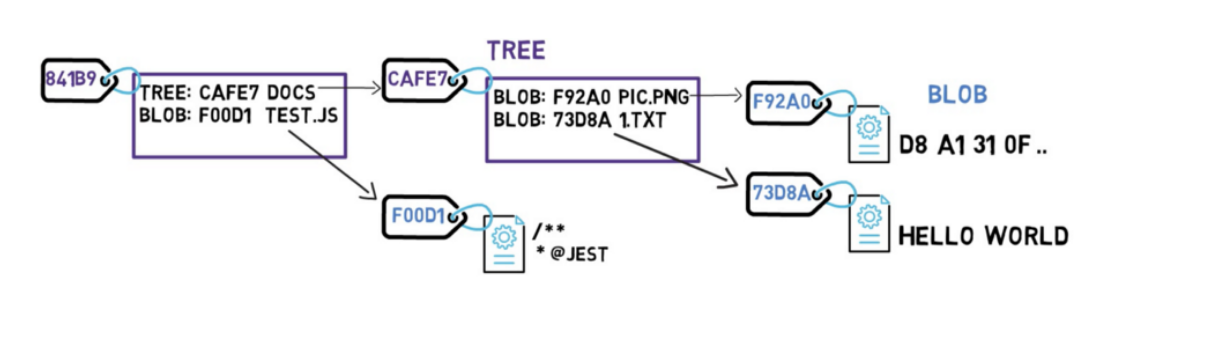
\includegraphics[width=1\linewidth]{img/tree-blobs}
		\label{fig:tree-blobs}
	\end{figure}
\end{frame}

\begin{frame}{Git Internals - Commit}
\begin{figure}
	\centering
	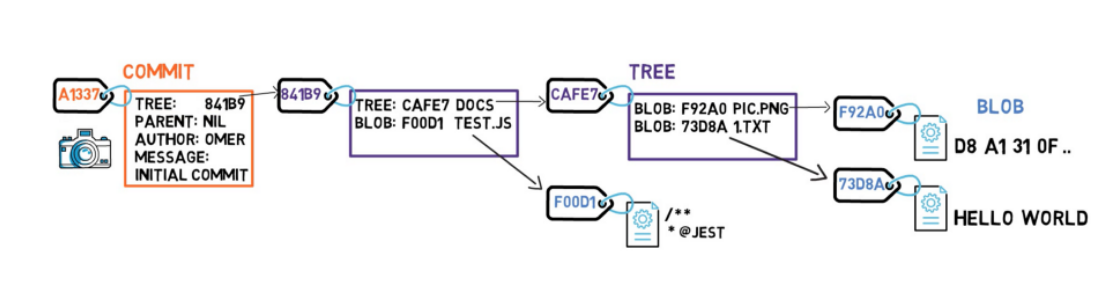
\includegraphics[width=1\linewidth]{img/tree-blobs1}
	\label{fig:tree-blobs1}
\end{figure}
\end{frame}

\begin{frame}[plain]{Links interesantes}
	\begin{itemize}
		\item \href{https://git-scm.com/book/es/v2/Los-entresijos-internos-de-Git-Los-objetos-Git}{Los objetos de Git}
	\end{itemize}
\end{frame}

\end{document}
